

We begin by establishing the necessary notations and definitions.

\subsection{Statistical risks in support recovery problems}
\label{subsec:risks}

\begin{figure}
      \centering
      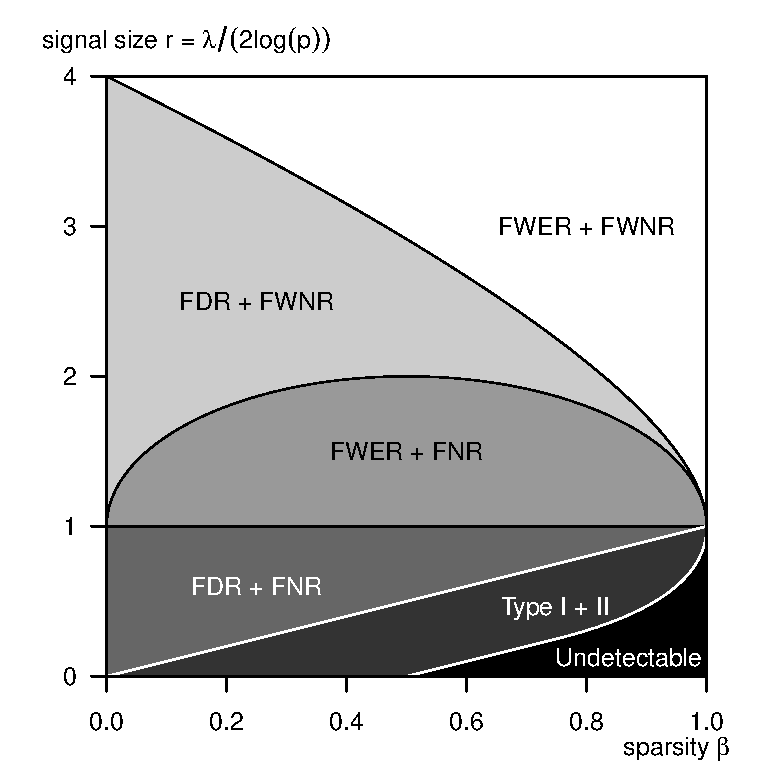
\includegraphics[width=0.6\textwidth]{phase_diagram_chisquared_ALL_boundaries.eps}
      % \includegraphics[width=0.35\textwidth]{phase_diagram_chisquared.eps}
      \caption{The phase diagram for the high-dimensional chi-square model \eqref{eq:model-chisq}, illustrating the boundaries of the exact support recovery (FWER + FWNR; top curve; Theorem \ref{thm:chi-squared-exact-boundary}),
      the approximate-exact support recovery (FDR + FWNR; second curve from top; Theorem \ref{thm:chi-squared-approx-exact-boundary}),
      the exact-approximate support recovery (FWER + FNR; horizontal line $r=1$; Theorem \ref{thm:chi-squared-exact-approx-boundary}),
      and the approximate support recovery problems (FDR + FNR; tilted line $r=\beta$; Theorem \ref{thm:chi-squared-approx-boundary}).
      The signal detection problem (type I + type II errors of the global test; lower curve) was studied in \citep{donoho2004higher}. 
      In each region of the diagram and above, the annotated statistical risk can be made to vanish, as dimension $p$ diverges. 
      Conversely, the risks has liminf at least one.
      All boundaries are unaffected by the degree-of-freedom.
      All boundaries are identical to those in the Gaussian additive error model \eqref{eq:model-additive} under one-side alternatives; see Section \ref{sec:additive-error-model-boundaries}.
    %   , setting $\lambda=\mu^2$.
      } 
      \label{fig:phase-chi-squared}
\end{figure}

Recall that in support recovery problems, our goal is to come up with a procedure, denoted $\mathcal R$, that produces a set estimate $\widehat{S}$ of the true index set of relevant variables  $S=\{i:\lambda(i)\neq 0\}$.
Formally, one should write $\widehat{S}(\mathcal{R}(x))$ to reflect the dependence of the set estimate on the procedure $\mathcal{R}$ and on the test statistics $x$; 
for notational convenience, we suppress this dependence and simply write $\widehat{S}$.
% in place of $\widehat{S}(\mathcal{R}(x))$ 

For a given procedure $\mathcal{R}$, the \emph{false discovery rate} (FDR) 
and the \emph{false non-discovery rate} (FNR) of a procedure is defined as
% of the procedure is defined to be the expected fraction of false findings not in the true index set, among the reported discoveries \cite{benjamini1995controlling}. 
% Its counterpart, \emph{false non-discovery rate} (FNR), measuring the power of the procedure, is defined as the expected fraction of missed detection. 
% Mathematically, we define
\begin{equation} \label{eq:FDR-FNR}
    \mathrm{FDR}(\mathcal{R}) = \E\left[\frac{|\widehat{S}\setminus S|}{\max\{|\widehat{S}|,1\}}\right],
    \quad \text{and} \quad
    \mathrm{FNR}(\mathcal{R}) = \E\left[\frac{|S\setminus \widehat{S}|}{\max\{|{S}|,1\}}\right],
\end{equation}
where the maxima in the denominators resolve the otherwise division by 0 problem. 
Roughly speaking, FDR measures the expected fraction of false findings, while FNR describes the proportion of type II errors among the true signals, and reflects the average marginal power of the procedure.

A more stringent criterion for false discovery is the family-wise error rate (FWER),
% defined to be the probability of reporting at least one finding not contained in the true index set.
and correspondingly, a more stringent criteria for false non-discovery is the family-wise non-discovery rate (FWNR), i.e.,
% the probability of missing at least one signal in the true index set. That is,
\begin{equation} \label{eq:FWER-FWNR}
    \mathrm{FWER}(\mathcal{R}) = 1 - \P[\widehat{S} \subseteq S], 
    \quad \text{and} \quad
    \mathrm{FWNR}(\mathcal{R}) = 1 - \P[S \subseteq \widehat{S}].
\end{equation}

We introduce five different ways to quantified statistical risks in support recovery problems, leading to different asymptotic limits. 
Following \cite{arias2017distribution}, we define the risk for \emph{approximate} support recovery as
\begin{equation} \label{eq:risk-approximate}
    \mathrm{risk}^{\mathrm{A}}(\mathcal{R}) = \mathrm{FDR}(\mathcal{R}) + \mathrm{FNR}(\mathcal{R}).
\end{equation}
Analogously, we define the risk for \emph{exact} support recovery as
\begin{equation} \label{eq:risk-exact}
    \mathrm{risk}^{\mathrm{E}}(\mathcal{R}) = \mathrm{FWER}(\mathcal{R}) + \mathrm{FWNR}(\mathcal{R}).
\end{equation}
An intimately related measure of success in the exact support recovery risk is the probability of exact recovery, 
\begin{equation} \label{eq:risk-prob}
    \P[\widehat{S} = S] = 1 - \P[\widehat{S} \neq S].
\end{equation}
The relationship between $\P[\widehat{S} = S]$ and $\mathrm{risk}^{\mathrm{E}}$ will be analyzed in Section \ref{subsec:asymptotics}.

The discussion in Section \ref{subsec:asymmetric-risk} --- and in particular, the GWAS application --- prompts us to consider risks that weigh both the family-wise error rate and the marginal power of discovery.
One such risk metric is what we refer to as the \emph{exact-approximate} support recovery risk
\begin{equation} \label{eq:risk-exact-approx}
    \mathrm{risk}^{\mathrm{EA}}(\mathcal{R}) = \mathrm{FWER}(\mathcal{R}) + \mathrm{FNR}(\mathcal{R}).
\end{equation}
The somewhat strange name is chosen to reflect ``exact false discovery control, and approximate false non-discovery control'', should the risk metric \eqref{eq:risk-exact-approx} vanish asymptotically.

Analogously, we consider the \emph{approximate-exact} support recovery risk
\begin{equation} \label{eq:risk-approx-exact}
    \mathrm{risk}^{\mathrm{AE}}(\mathcal{R}) = \mathrm{FDR}(\mathcal{R}) + \mathrm{FWNR}(\mathcal{R}),
\end{equation}
which places more emphasis on non-discovery control.

% These two risks differ in their stringency in controlling false discovery and false non-discovery.
Theoretical limits and performance of procedures in support recovery problems will be studied in terms of the five risk metrics \eqref{eq:risk-approximate}, \eqref{eq:risk-exact}, \eqref{eq:risk-prob}, \eqref{eq:risk-exact-approx} and \eqref{eq:risk-approx-exact}, defined above.

\subsection{Thresholding procedures}
\label{subsec:thresholding-procedures}

We shall study the performance of five procedures,
all of which belong to the broad class of thresholding procedures.
\begin{definition}[Thresholding procedures]
A thresholding procedure for estimating the support 
$S:=\{i\, :\, \lambda(i)\neq0\}$ is one that takes on the form
\begin{equation} \label{eq:thresholding-procedure}
    \widehat{S} = \left\{i\,|\,x(i) \ge t(x)\right\},
\end{equation}
where the threshold $t(x)$ may depend on the data $x$.
\end{definition}
Examples of thresholding procedures include ones that aim to control FWER --- Bonferroni's \cite{dunn1961multiple}, Sid\'ak's \citep{vsidak1967rectangular}, Holm's \citep{holm1979simple}, and Hochberg's procedure \citep{hochberg1988sharper} --- as well as procedures that target FDR, such as the Benjamini-Hochberg \cite{benjamini1995controlling} and the Cand\'es-Barber procedure \cite{barber2015controlling}.
Indeed, thresholding procedures \eqref{eq:thresholding-procedure} is such a general class that it contains most (but not all) of the statistical procedures in the multiple testing literature.
% \cite{roquain2011type}.

We shall restrict our attention to the class of thresholding procedures.
Specifically, the lower bounds that we develop in Theorems \ref{thm:chi-squared-exact-boundary} through \ref{thm:chi-squared-approx-exact-boundary}, and in Theorems \ref{thm:additive-error-exact-approx-boundary} and \ref{thm:additive-error-approx-exact-boundary} below, are only meant to apply to such procedures. 
The optimality of thresholding procedures and the consequences of this restriction will be briefly discussed in Section \ref{sec:discussions}.

\subsection{Asymptotic success and failure of support recovery}
\label{subsec:asymptotics}

We shall work under the asymptotic regime where the problem dimension $p$ diverges.
Specifically, we will work with the triangular array of chi-square models \eqref{eq:model-chisq} indexed by $p$.
Let the non-centrality parameter vectors $\lambda = \lambda_p$ have 
\begin{equation} \label{eq:signal-sparsity}
    |S_p| = \left\lfloor p^{1-\beta} \right\rfloor, \quad \beta\in(0,1)
\end{equation}
non-zero entries, where $\beta$ parametrizes the problem sparsity.
The closer $\beta$ is to 1, the sparser the support $S$; conversely, when $\beta$ is close to 0, the support is dense with many non-null signals.

We further parametrize the range of the non-zero (and perhaps unequal) signals with
\begin{equation} \label{eq:signal-size}
    \underline{\Delta} = 2\underline{r}\log{p}
    \le \lambda(i) \le
    \overline{\Delta} = 2\overline{r}\log{p}, \quad \text{for all}\;\;i\in S_p,
\end{equation}
for some constants $0<\underline{r}\le\overline{r}\le+\infty$.

\begin{remark}
\label{rmk:global-test-boundary}
The parametrization of signal sparsity \eqref{eq:signal-sparsity} and signal sizes  \eqref{eq:signal-size} in the chi-square model seem to be first introduced by \citet{donoho2004higher}, where the signal sizes were assumed equal with magnitude $(2{r}\log{p})$.
It was shown in \cite{donoho2004higher} that a phase transition in the $r$-$\beta$ plane exists for the signal detection problem. 
That is, if $r$ is above a so-called detection boundary, then the global null hypothesis $\lambda(i)=0$ for all $i=1,\ldots,p$ can be told apart from the alternative as $p\to\infty$ with vanishing type I and type II errors; 
otherwise, below the boundary, no test can do better than a random guess.
We shall see that the scaling of sparsity \eqref{eq:signal-sparsity} and signal size \eqref{eq:signal-size} is also suitable for studying the phase transitions of the support recovery problem.
\end{remark}

The criteria for success and failure in support recovery problems under this asymptotic regime are defined as follows.
\begin{definition} \label{def:exact-recovery-success-failure}
We say a sequence of procedures $\mathcal{R} = \mathcal{R}_p$ succeeds asymptotically in the exact (and respectively, exact-approximate, approximate-exact, and approximate) support recovery problem if 
\begin{equation} \label{eq:support-recovery-success}
    \mathrm{risk}^{\mathrm{P}}(\mathcal{R}) \to 0, \quad \text{as}\quad p\to\infty,
\end{equation}
where $\mathrm{P}=\mathrm{E}$ (respectively, $\mathrm{EA}$, $\mathrm{AE}$, $\mathrm{A}$).

Conversely, we say the exact support recovery fails asymptotically in the exact (and respectively, exact-approximate, approximate-exact, and approximate) support recovery problem if 
\begin{equation} \label{eq:support-recovery-faliure}
    \liminf\mathrm{risk}^{\mathrm{P}}(\mathcal{R}) \ge 1, \quad \text{as}\quad p\to\infty,
\end{equation}
where $\mathrm{P}=\mathrm{E}$ (respectively, $\mathrm{EA}$, $\mathrm{AE}$, $\mathrm{A}$).
\end{definition}
% Similarly, we define the criteria for asymptotic success and failure for approximate support recovery as follows.
% \begin{definition} \label{def:approx-recovery-success-failure}
% We say a sequence of procedures $\mathcal{R} = \mathcal{R}_p$ succeeds asymptotically in the approximate support recovery problem if 
% \begin{equation} \label{eq:approx-recovery-success}
%     \mathrm{risk}^{\mathrm{A}}(\mathcal{R}) \to 0, \quad \text{as}\quad p\to\infty.
% \end{equation}
% We say the approximate support recovery fails asymptotically if 
% \begin{equation} \label{eq:approx-recovery-failure}
%     \liminf\mathrm{risk}^{\mathrm{A}}(\mathcal{R}) \ge 1, \quad \text{as}\quad p\to\infty.
% \end{equation}
% \end{definition}

% The performance of procedures in terms of the criteria in Definition \ref{def:exact-recovery-success-failure} 
% % and \ref{def:approx-recovery-success-failure} 
% will be analyzed in Sections \ref{subsec:exact-support-recovery-boundary} and \ref{subsec:approx-support-recovery-boundary}.

We now elaborate on the relationship between the probability of exact recovery and risk of exact support recovery, as promised in Section \ref{subsec:risks}.
\begin{lemma} \label{lemma:risk-exact-recovery-probability}
Let $\mathcal{R} = \mathcal{R}_p$ be the sequence of procedures for support recovery under the chi-square model \eqref{eq:model-chisq}. 
%The probability of exact recovery $\P[\widehat{S} = S]$, and risk of exact support recovery $\mathrm{risk}^{\mathrm{E}}$, defined in \eqref{eq:risk-exact}, are related as follows,
In this case, as $p\to\infty$, we have
\begin{equation} \label{eq:exact-recovery-implies-risk-0}
    \P[\widehat{S} = S] \to 1 \iff \mathrm{risk}^{\mathrm{E}}\to0,
\end{equation}
and
\begin{equation} \label{eq:failure-recovery-implies-risk-1}
    \P[\widehat{S} = S] \to 0 \implies \liminf\mathrm{risk}^{\mathrm{E}}\ge1,
\end{equation}
where the dependence on $p$ was suppressed for notational convenience.
\end{lemma}


By virtue of Lemma \ref{lemma:risk-exact-recovery-probability}, it is sufficient to study the probability of exact support recovery $\P[\widehat{S}=S]$ in place of $\mathrm{risk}^{\mathrm{E}}$, if we are interested in the asymptotic properties of the risk in the sense of \eqref{eq:support-recovery-success} and \eqref{eq:support-recovery-faliure}.
% (The converse, discussed in Section \ref{sec:discussions} below, is not true.)
